\documentclass[main.tex]{subfiles}
\begin{document}

\section*{How to play the game}


\subsection*{Putting together the game}
\begin{enumerate}
\item Print out the game.
\item Glue together the pages two by two, back to back.
\item Cut out the individual cards.
\end{enumerate}

\subsection*{Preparation}
\begin{enumerate}
\item Shuffle the cards
\item Put the cards info-down on the table in one pile.
\end{enumerate}

\subsection*{Playing the game}
The game is turn-based and is played with at least two people.
The player who can list the network layers the fastest, from top to bottom and back up, gets the first turn.

\begin{figure}[H]
    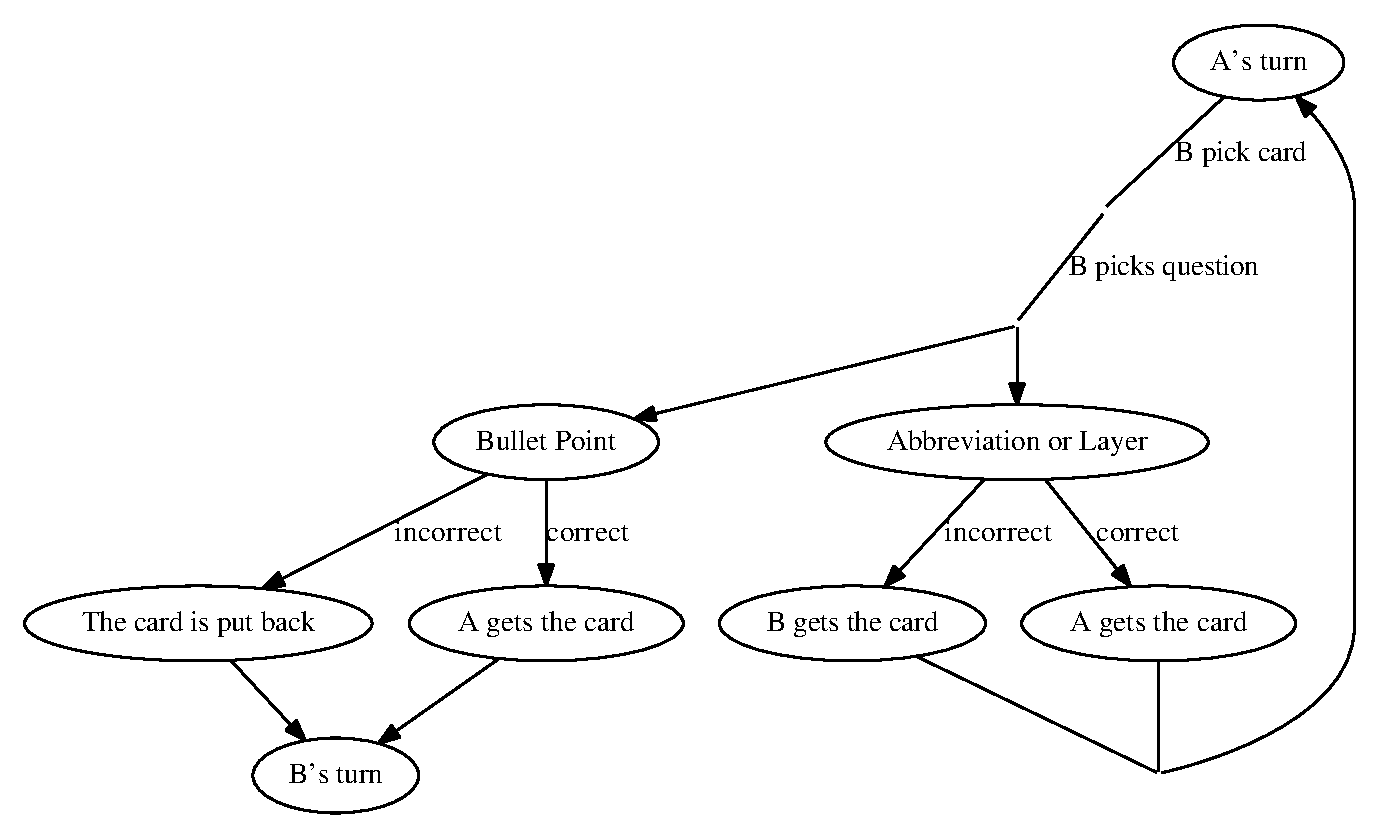
\includegraphics[width=\textwidth]{rules.eps}
\end{figure}

\end{document}

%%% Local Variables:
%%% mode: latex
%%% TeX-master: t
%%% End:
